\documentclass[12pt,letterpaper]{article}
\usepackage[utf8]{inputenc}
\usepackage[spanish]{babel}
\usepackage{graphicx}
\usepackage[left=2cm,right=2cm,top=2cm,bottom=2cm]{geometry}
\usepackage{graphicx} % figuras
% \usepackage{subfigure} % subfiguras
\usepackage{float} % para usar [H]
\usepackage{amsmath}
\usepackage{array}
%\usepackage{txfonts}
\usepackage{stackrel} 
\usepackage{multirow}
\usepackage{enumerate} % enumerados
\renewcommand{\labelitemi}{$-$}
\renewcommand{\labelitemii}{$\cdot$}
% \author{}
% \title{Caratula}

\begin{document}

% Fancy Header and Footer
% \usepackage{fancyhdr}
% \pagestyle{fancy}
% \cfoot{}
% \rfoot{\thepage}
%

% \usepackage[hidelinks]{hyperref} % CREA HYPERVINCULOS EN INDICE

% \author{}
\title{Proyecto Base de Datos}

\begin{titlepage}
\begin{center}
\begin{figure}[htb]
\begin{center}

\includegraphics[width=3.5cm]{./img/logo}
\end{center}
\end{figure}

\vspace*{0.15in}
\begin{Large}
\textbf{UNIVERSIDAD PRIVADA DE TACNA}\\
\end{Large}

\vspace*{0.1in}
\begin{Large}
\textbf{FACULTAD DE INGENIERIA} \\
\end{Large}

\vspace*{0.1in}
\begin{Large}
\textbf{ESCUELA PROFESIONAL DE INGENIERIA DE SISTEMAS} \\
\end{Large}

\vspace*{0.3in}
\begin{Large}
\textbf{TITULO:}\\
\end{Large}

\vspace*{0.1in}
\begin{Large}
Sistema de Seguridad JeaNet \\
\end{Large}

\vspace*{0.2in}
\begin{Large}
\textbf{CURSO:} \\
\end{Large}

\vspace*{0.1in}
\begin{large}
BASE DE DATOS II\\
\end{large}

\vspace*{0.2in}
\begin{Large}
\textbf{DOCENTE:} \\
\end{Large}

\vspace*{0.1in}
\begin{large}
Ing. Patrick José Cuadros Quiroga\\
\end{large}

\vspace*{0.2in}
\vspace*{0.1in}
\begin{large}
Integrantes: \\
\begin{flushleft}
Arias La Torre, José Luis 			\hfill	(2017059559) \\
Cancino Tapia, Luis Antonio 		\hfill	(2015052383) \\
Crispín Huamaní, Angel Alberto      \hfill	(2017059468) \\
Gutierrez Ponce, José Carlos  		\hfill	(2017059277) \\
Zuñiga Silva, Roby Gerson       	\hfill	(2015052684) \\

\end{flushleft}
\end{large}
\vspace*{0.1in}
\begin{large}
Tacna - Perú\\
\end{large}
\vspace*{0.1in}
\begin{large}
2020\\
\end{large}

\end{center}

\end{titlepage}

\include{Secciones/articulo}
%%%%%%%%%%%%%%%%%%%%%%%%%%%%%%%%%%%%%%%%%%%%%%%%%%%%%%%%%
\newpage
\tableofcontents

\newpage
\begin{LARGE}
    \begin{center}
        \textbf{Sistema de Seguridad JeaNet} \\
    \end{center}
\end{LARGE}
\vspace*{0.1in}
\textbf{Resumen}\\
Una base de datos constituye un sistema que permite un manejo adecuado de los datos, garantizando la seguridad e integridad de estos y permitiendo el acceso a distintos usuarios de forma transparente. La base de datos está formada por los datos en sí, organizados de forma estructurada, mientras que las operaciones las provee el sistema gestor de base de datos (SGBD).
Existen diversos modelos para el almacenamiento de datos, siendo el modelo relacional el más habitual en la actualidad. En el modelo relacional la información se organiza en tablas relacionadas entre sí. Cada fila de una base de datos conforma una tupla, que contiene la información correspondiente a una entidad dada.
El diseño de la base de datos es de gran importancia, y conlleva el diseño de un modelo conceptual, el diseño de un modelo físico, la implementación y el mantenimiento. Herramientas como los diagramas E--R son de ayuda en las fases de diseño, cuyo principal objetivo es crear una estructura de la base de datos que facilite la interpretación de la información contenida y permita sacar el máximo rendimiento de esta.
En lo que a los SIG respecta, las bases de datos se han ido incorporando paulatinamente a la gestión de los datos espaciales. Partiendo de una situación inicial en la que no se empleaban sistemas gestores de bases de datos, estos han ido integrándose en los SIG de diversas formas. En la actualidad, se emplean bases de datos relacionales, que son adaptadas para poder almacenar datos espaciales y poder realizar operaciones sobre ellos. Los SGBD extensibles representan la última tendencia, y en ellos puede integrarse plenamente la información geográfica de forma óptima.
\\

\textbf{Abstract}\\
A database constitutes a system that allows an adequate handling of the data, guaranteeing the security and integrity of these and allowing access to different users in a transparent way. The database is made up of the data itself, organized in a structured way, while the operations are provided by the database management system (DBMS).
There are several models for data storage, the relational model being the most common today. In the relational model the information is organized in related tables. Each row in a database forms a tuple, which contains the information corresponding to a given entity.
The design of the database is of great importance, and involves the design of a conceptual model, the design of a physical model, implementation and maintenance. Tools such as E - R diagrams are helpful in the design phases, the main objective of which is to create a database structure that facilitates the interpretation of the information contained and allows to get the most out of it.
As far as GIS is concerned, databases have been gradually incorporated into the management of spatial data. Starting from an initial situation in which database management systems were not used, these have been integrated into GIS in various ways. At present, relational databases are used, which are adapted to be able to store spatial data and be able to perform operations on them. Extensible DBMS represent the latest trend, and geographic information can be optimally integrated into them.
\\
\newpage
\begin{LARGE}
    \begin{center}
        \textbf{Sistema de Seguridad JeaNet} \\
    \end{center}
\end{LARGE}
\vspace*{0.1in}
\section{Antecedentes o introducción}
El desarrollo tecnológico de nuestra sociedad ha traído la informatización de todas las empresas, negocios, educación, la administración pública, transportes, etc. Esto ha supuesto tener que crear programas informáticos para realizar las tareas que antes se hacían manualmente. Estos programas manejaban datos de entrada y producían datos en su salida. Pero los datos debían de almacenarse de alguna manera para que los programas pudieran acceder a ellos y manejarlos sin provocar errores. Todas estas necesidades hicieron que algunas personas y empresas comenzaran a investigar cómo poder solventar todos estos problemas. Se crearon modelos de datos que permitían representar la información real que debía ser informatizada.
Hoy en día la información es la base de nuestra sociedad, recibimos y manejamos volúmenes enormes de información y el ordenador es la herramienta que nos permite almacenar y tratar esa información.
Para poder guardar y recuperar esa información necesitamos de un sistema de almacenamiento que sea fiable, fácil de manejar, eficiente, y de aplicaciones capaces de llevar a cabo esa tarea y de obtener resultados a partir de la información almacenada.
Este sistema es el denominado Sistema Gestor de Base de Datos  y consiste en un conjunto de datos relacionados entre sí y un conjunto de programas desarrollados para gestionar esos datos y comprobar que el sistema se mantenga libre de errores. Además aplicaciones de usuario que accedan a la base de datos para utilizar esa información. La inmensa mayoría de bases de datos que existen en el mercado hoy en día son bases de datos relacionales, bases de datos que organizan la información en tablas relacionadas entre sí mediante campos de relación y que cumplen una serie de reglas que procuran evitar redundancia y asegurar la integridad de los datos almacenados en ellas así como la seguridad de los datos


\section{Titulo}
Sistema de Seguridad Jeanet

\section{Autores}
\begin{itemize}
	\item Arias Flores, José Luis  
	\item Cancino Tapia, Luis Antonio 
	\item Crispin Huamani, Angel Alberto
	\item Gutierrez Ponce, Jose Carlos
	\item Zuñiga Silva, Robi Gerson
\end{itemize}

\section{Planteamiento del problema}
    \subsection{Problema}
    Los Productos Software, sistemas y/o aplicaciones son creadas, desarrolladas e implementadas por seres humanos y por ende en cualquiera de sus etapas de creación se puede presentar una equivocación, al generarse esa “Equivocación” se puede conllevar a un defecto en el software, por ejemplo mala digitación, distracción al codificar, mala elaboración de un documento entre otras. Si no se ha identificado ese defecto y el software o la aplicación se ejecuta, hay un alto riesgo de que la aplicación no haga lo que debería hacer o el objeto para lo cual fue creada, es decir se genera un fallo o desperfecto
    El proyecto realizado en el V ciclo del curso de Programacion II se técnicas,métodos y/o practicas “equivocadas”.
    
    \subsection{Justificación}
    El aseguramiento de la calidad debe ser parte integral en cualquier proyecto de software. La ciencia detrás de las pruebas está en identificar con precisión la calidad del software con el objetivo de asegurar que el software funcione como se espera que funcione en todo momento. El término se refiere a diferentes métodos y procesos para probar software y garantizar su calidad.
    En este proyecto veremos mejoras de calidad aplicadas a un proyecto realizado en el V ciclo del curso de Programación II

    \subsection{Alcance}
    Conocer y aplicar las diferentes normas, procesos y procedimientos para garantizar la calidad de los productos software, aplicando las pruebas de calidad de software necesarias para que con ellas se pueda ayudar a reducir los riesgos en las aplicaciones, logrando que se identifiquen los defectos antes de que se ejecuten, así de forma proactiva tomar decisiones que permitan  hacer las actividades necesarias para mejorar las condiciones del software y ofertar un producto que satisfaga las necesidades del cliente.

\section{Objetivos}
    \subsection{General}
    Mejorar la calidad del software que fue creado en el V Ciclo en el curso de Programación II de la Universidad Privada de Tacna
    \subsection{Específicos}
    Aprender a usar mejores técnicas de programación
    Usar herramientas que ayuden a mejorar la calidad(SONARQUBE)

\section{Referentes teóricos}
    \subsection{¿Cómo se estructuran las bases de datos relacionales?}
    El modelo relacional significa que las estructuras lógicas de datos las tablas de datos, vistas e índices están separadas de las estructuras físicas de almacenamiento. Esta separación significa que los administradores de bases de datos pueden administrar el almacenamiento físico de datos sin afectar el acceso a esos datos como una estructura lógica. Por ejemplo, cambiar el nombre de un archivo de base de datos no cambia el nombre de las tablas almacenadas en él. \\
    La distinción entre lógica y física también se aplica a las operaciones de la base de datos, que son acciones claramente definidas que permiten a las aplicaciones manipular los datos y las estructuras de la base de datos. Las operaciones lógicas permiten que una aplicación especifique el contenido que necesita, mientras que las operaciones físicas determinan cómo se debe acceder a esos datos y luego realizan la tarea.\\
    Para garantizar que los datos sean siempre precisos y accesibles, las bases de datos relacionales siguen ciertas reglas de integridad. Por ejemplo, una regla de integridad puede especificar que no se permitan filas duplicadas en una tabla, para eliminar la posibilidad de que ingrese información errónea en la base de datos.\\

    \subsection{¿Qué es un modelo relacional?}
    En los primeros años de las bases de datos, cada aplicación almacenaba datos en su propia estructura única. Cuando los desarrolladores querían crear aplicaciones para usar esos datos, tenían que saber mucho sobre la estructura de datos particular para encontrar los datos que necesitaban. Estas estructuras de datos eran ineficientes, difíciles de mantener y difíciles de optimizar para ofrecer un buen rendimiento de la aplicación. El modelo de base de datos relacional se diseñó para resolver el problema de varias estructuras de datos arbitrarias.\\
    El modelo relacional proporcionó una forma estándar de representar y consultar datos que cualquier aplicación podría utilizar. Desde el principio, los desarrolladores reconocieron que la principal fortaleza del modelo de base de datos relacional estaba en el uso de tablas, que eran una forma intuitiva, eficiente y flexible de almacenar y acceder a información estructurada.\\
    Con el tiempo, cuando los desarrolladores comenzaron a utilizar el lenguaje de consulta estructurado (SQL) para escribir y consultar datos en una base de datos, surgió otra fortaleza del modelo relacional. Durante muchos años, se utilizó ampliamente el SQL como lenguaje para consultas de bases de datos. El SQL, que se basa en el álgebra relacional, proporciona un lenguaje matemático internamente consistente que facilita la mejora del rendimiento de todas las consultas de la base de datos. En comparación, otros enfoques deben definir consultas individuales.\\

    \subsection{¿Cuáles son los beneficios de las bases de datos relacionales?}
    Las organizaciones de todo tipo y tamaño utilizan el modelo relacional simple pero poderoso para una amplia variedad de necesidades de información. Las bases de datos relacionales se utilizan para hacer seguimiento de los inventarios, procesar transacciones de comercio electrónico, administrar grandes cantidades de información de clientes de misión crítica y mucho más. Se puede considerar una base de datos relacional para cualquier necesidad de información en la que los puntos de datos se relacionen entre sí y se deban administrar de una manera segura, consistente y basada en reglas.\\
    Las bases de datos relacionales existen desde la década de 1970. Actualmente, las ventajas del modelo relacional continúan convirtiéndolo en el modelo más aceptado para bases de datos.\\
    
    \subsection{¿Qué contiene un Diccionario de Datos?}
    No podría hablarte de un estándar puesto que, dependiendo de las necesidades o formatos, podemos encontrar varios en diferentes lugares.\\
    Algunas documentaciones incluyen dentro del llamado Diccionario de Datos al Modelo Entidad Relación, su gráfica y una descripción de todas las relaciones que puedan existir.\\
    No considero que exista una sola respuesta, así que dejaré un poco abierto este punto a criterio de cada uno e impulsando puedas buscar mucha más información en todo lo que es documentación de software.\\
    
    \subsection{¿Qué es un ORM?}
    Object Relational mapping, o lo que es lo mismo, mapeo de objeto relacional, es un modelo de programación que consiste en la transformación de las tablas de una base de datos, en una serie de entidades que simplifiquen las tareas básicas de acceso a los datos para el programador.\\
    Desde hace muchos años el lenguaje más usado para acceder a las bases de datos relacionales ha sido el SQL. \\
    
    \subsection{¿Por qué usar un ORM?}
    Aunque el lenguaje SQL se usa para acceder a muchas de las bases de datos existentes, existen múltiples varianzas en las funciones que los distintos SGBD han usado. Un ejemplo muy sencillo sería delimitar el número de registros de una consulta:\\

    \textit{SELECT TOP 10 * FROM usuarios //SqlServer}\\
    \textit{SELECT * FROM usuarios LIMIT 10 //MySQL}\\
    \textit{SELECT * FROM usuarios WHERE rownum<=20; //Oracle}\\
    
    Tres de las bases de datos más importantes, y como veis, para algo tan fácil vemos diferencias. Esto para el programador supone tener que conocer el lenguaje para cada Base de datos, y más importante aún, si en un futuro se desea migrar la aplicación, habría que reescribir gran número de las consultas.\\
    Esto el ORM al tener un capa intermedia, abstrae al programador de la base de datos y le centra en el desarrollo de la aplicación.\\
    Otro punto importante es la facilidad de trabajo, un ORM, nos facilita las labores básicas de cualquier acceso a datos , el CRUD (Create, Read, Update y Delete). Realizando todas estas labores a través de un lenguaje de alto nivel orientado a objetos. \\
    
    \subsection{¿Qué son las pruebas?}
    Antes de ver una definición de prueba, veremos la percepción que tienen los desarrolladores acerca de las pruebas. Según [MYE11], los desarrolladores siguen las siguientes definiciones que llevan a una percepción falsa:
    \\
    \\
    •	“Las pruebas son el proceso de demostrar que no hay errores presentes”.
    \\
    \\
    •	“El propósito de las pruebas es demostrar que un programa realiza las funciones indicadas correctamente”.
    \\
    \\
    •	“Las pruebas son el proceso de establecer confianza en que un programa hace lo que se supone que debe hacer” .
    Jhon Myers indica que estas definiciones están mal planteadas. Cuando probamos un programa se quiere aportar un valor añadido a lo que estamos probando, elevar la calidad y fiabilidad y esto nos lleva a tener que encontrar y eliminar los errores en el programa.
    Esto quiere decir que no tenemos que probar un programa para demostrar que funciona, sino que tenemos que partir de la suposición de que el programa va a contener errores. La definición de prueba que aporta Myers es:
    \\
    \\
    •	“La prueba es el proceso de ejecución de un programa con la intención de encontrar errores”.
    Pero, ¿por qué se toma esta definición como válida y las anteriores no?.
    
    Si tomamos la primera definición mencionada - “El testing es el proceso de demostrar que no hay errores presentes”, psicológicamente estaremos dirigidos hacia esa meta y tenderemos a seleccionar los casos de prueba con una baja probabilidad de causar que el programa falle. Si por el contrario tomamos como objetivo demostrar que un programa tiene fallos, tendremos una mayor probabilidad de encontrar errores.
    Si tomáramos la definición de “Testing es el proceso de establecer confianza en que un programa hace lo que se supone que debe hacer” estaríamos dando por sentado que un programa que hace lo que se supone debe hacer, no tiene errores y eso es un error ya que, aunque el programa realice su función, puede contener errores.
    El ISTQB (International Software Tesng Qualifications Board), una organización sin ánimo de lucro creada en el año 2002 por empresas, instituciones, organizaciones y personas especializadas en el campo de las pruebas y la industria del software, define las pruebas como [ISTQB]:
    “El proceso que consiste en todas las actividades del ciclo de vida, tanto estáticas como dinámicas relacionadas con la planificación, preparación y evaluación de productos de software y productos relacionados con el trabajo para determinar que cumplen los requisitos especificados, para demostrar que son aptos para el propósito y para detectar defectos”.
    Cem Kaner, profesor de Ingeniería de software en el instituto tecnológico de Florida, es uno de los defensores y principales gurús de las pruebas de software, las define como 
    \\
    \\
    •	“Las pruebas de software son la investigación empírica y técnica realizada para facilitar a los interesados información sobre la calidad del producto o servicio bajo pruebas”.
    Kaner introduce la figura del técnico que mediante la investigación aportará datos sobre la calidad del producto y no se centrará únicamente en la detección del fallo.
    Edsger W. Dijstra, científico de la computación entre cuyas contribuciones a la ciencia esta ‘la solución del problema del camino más corto’, también conocido como el algoritmo de Dijstra, define el proceso de pruebas como [WEB03]:
    \\
    \\
    •	“Las pruebas de software pueden ser una manera muy eficaz de mostrar la presencia de errores, pero son totalmente inadecuadas  para mostrar su ausencia.”
    Todas y cada una de estas definiciones tienen algo en común, todas se centran en mayor o menor manera en la detección de errores.
    Para terminar de entender las pruebas debemos diferenciar los términos error, fallo y defecto. Estos conceptos están relacionados entre si, pero tienen significados diferentes. Para comprender estas palabras y por ende las pruebas, vamos a ver como las define el ISTQB:
    “Una persona puede cometer un error que a su vez puede producir un defecto en el código de programa o en un documento. Si se ejecuta un defecto en el código, el sistema puede no hacer lo que debiera (o hacer algo que no debiera), lo que provocaría un fallo. Algunos defectos de software pueden dar lugar a fallos, pero no todos los defectos lo hacen.”
    Así pues tenemos:
    \\
    \\
    •	\textbf{Error:} está provocado por la acción humana, por ejemplo el error lo provocará el desarrollador que realizará una incorrecta interpretación de un método del programa que producirá un resultado no esperado.
    \\
    \\
    •	\textbf{Defecto:} provocado por un error de implementación, por ejemplo el defecto lo provocará el haber utilizado el operador “x + y > z” en vez de “x + y => z”
    \\
    \\
    •	\textbf{Fallo:} al ejecutar el programa con un defecto obtendremos resultados no deseados, por ejemplo, cuando el resultado de la suma de los dos componentes fuese igual, no obtendríamos los mismos resultados al compararlos con las sentencias indicadas anteriormente. En sistemas muy complejos, como pueden ser una lanzadera espacial o una central eléctrica, pueden llegar a producir efectos catastróficos.
    
    \subsection{¿Por qué son importantes las pruebas?}

    Hoy en día, forman parte de nuestras vidas multitud de sistemas que contienen software, como por ejemplo los coches, smartphones, sistemas de producción de energía, programas bancarios, etc.
    \\
    \\
    Para responder a la pregunta anterior vamos a ver una serie de sucesos ocurridos durante el siglo XX, que ejemplifican lo importante que puede llegar a  ser probar el software antes de ponerlo en producción:
    \\
    \\
    •	El lanzamiento de la lanzadera Ariane-5 vuelo 501 (1996) fue considerado uno de los fallos de programación más caros de la historia hasta ese momento, sólo la carga que llevaba tenía un valor de 500 millones de dólares. Fue un cohete lanzado por la ESA (European Space Agency’s o agencia espacial europea) destruido aproximadamente a los 40 segundos  de ser lanzado. Según el informe de la ESA , el fallo de la Ariane 501 fue causado por la completa pérdida de guía e información de orientación treinta y siete segundos después del comienzo de la secuencia de ignición del motor principal. Esta pérdida de información se debió a errores de especificación y diseño en el software del sistema de referencia inercial. Las extensas revisiones y test llevados a cabo durante el programa de desarrollo del Ariane-5 no incluyeron el adecuado análisis y prueba del sistema de referencia inercial o del sistema de control de vuelo completo, lo cual podría haber detectado los fallos potenciales .
    \\
    \\
    •	El lanzamiento de la sonda Mariner 1 de la NASA (1962), tuvo que ser abortado por un fallo de software que afectaba a la trayectoria del cohete. El cohete fue destruido antes de que soltara la sonda que transportaba, ya que corría peligro de estrellarse en las rutas marítimas del atlántico norte. El coste aproximado del proyecto de la sonda Mariner 1 fue de 554 millones de dólares [WEB06].
    \\
    \\
    •	Therac 25, una máquina de radioterapia producida por la Atomic Energy of Canada Limited (AECL) en 1985, fue la causante de la muerte de tres personas directamente y otras tres sufrieron graves daños por la
    
    administración de sobredosis masivas de radiación. Una de las razones de que se produjera esta sobredosis fue un mal diseño del software, el código fuente no había sido revisado de forma independiente.
    \\
    \\
    •	Thomas Nicely, de la Universidad de Lynchburg, descubrió un error en la unidad de coma flotante del Pentium en 1994. El divisor en la unidad de coma flotante contaba con una tabla de división incorrecta, donde faltaban cinco entradas sobre mil, que provocaba errores de redondeo. Aunque el error afectaba a pocos usuarios, este hecho hizo mucho daño a la imagen  de Pentium y el costo total fue de 475 millones de dólares. Finalmente reemplazó los chips de todos los usuarios que lo solicitaron.
    \\
    \\
    •	En otoño de 1994, la compañía Disney lanzó su primer juego multimedia  en formato CD-ROM. Las ventas fueron enormes ya que fue uno de los juegos más comprados la navidad de ese año. El 26 de diciembre, el departamento de atención al cliente de Disney se vio desbordado por las llamadas de un gran número de usuarios descontentos que habían comprado el juego. Resulta que Disney no realizó pruebas en los diferentes modelos de PC disponibles en el mercado. Solo se realizaron pruebas sobre los PC que utilizaban los desarrolladores.
    \\
    \\
    Como se puede apreciar en los ejemplos anteriores, no probar adecuadamente el software, antes de ponerlo en producción, puede producir no sólo pérdidas económicas, sino también daños personales, llegando incluso a producir la muerte en algunos casos.
    A día de hoy el funcionamiento de casi todas las empresas depende en gran medida del software, ya sea por el sistema de finanzas de dicha empresa o por la maquinaria que lleva a cabo la fabricación de los productos, por lo que las empresas dependen del funcionamiento del software y de que éste pueda llegar a causar grandes fallos como los mencionados anteriormente que llevan a la pérdida de miles de millones de euros. No a todas las empresas les afectan de la misma
    \\
    \\
    manera los fallos producidos en el software, por lo que tenemos que evaluar los riesgos de éste, ya que pueden llegar a producir pérdidas irreparables.


    \subsection{¿Cuál es el objetivo de las pruebas?}

    El objetivo principal de las pruebas es aportar calidad al producto que se está desarrollando.
   
    \begin{center}
        \textit{Pero, ¿qué es calidad?}
    \end{center}
Este termino es definido por muchas organizaciones e ilustres en el mundo de la calidad de formas diferentes:
\\
\\
•	\textbf{ISO 9000} es un conjunto de normas sobre calidad y gestión de calidad, la define como “la calidad es el grado en el que un conjunto de características inherentes cumple con los requisitos” [WEB08].
\\
\\
•	\textbf{ISO 25000} es un conjunto de normas que tiene por objetivo la creación de un marco de trabajo común para evaluar la calidad del producto software, dice: “ la calidad es el grado en que el producto de software satisface las necesidades expresadas o implícitas, cuando es usado bajo condiciones determinadas” [WEB08].
\\
\\
•	\textbf{Philip Bayard Crosby}, que contribuyó a las prácticas de la gestión de la calidad, la define como “Conformidad con los requisitos” [WEB09].
\\
\\
•	\textbf{Armand V. Feigenbaum}, que diseñó el concepto del control total de la calidad, la define como “satisfacción de las expectativas del cliente” [WEB09].
\\
\\
•	\textbf{Genichi Taguchi}, que desarrolló una metodología para la aplicación de estadísticas para mejorar la calidad de los productos manufacturados, dice: “calidad es la pérdida (monetaria) que el producto o servicio ocasiona a la sociedad desde que es expedido” .
\\
\\
Podríamos seguir indicando definiciones de calidad de numerosos ilustres en el tema, en donde cada uno nos diría su definición y su manera de llegar a esta 
calidad. Hay dos puntos principales que tienen casi todas las definiciones de calidad: la satisfacción del cliente y el cumplimiento de los requisitos del producto.
La ISO 25010 , norma donde se trata la calidad del producto software, nos indica qué características tiene que tener un software para tener la calidad deseada:
\\
\begin{center}
	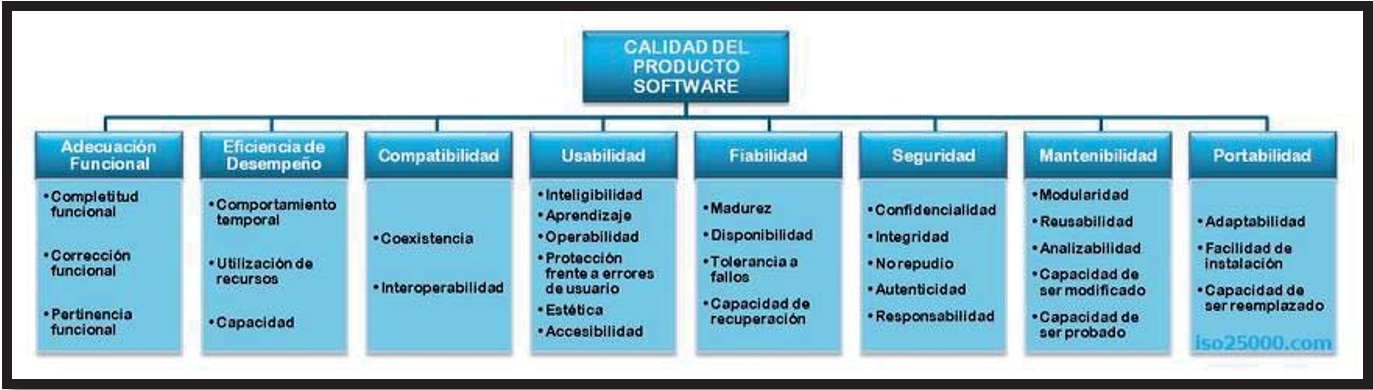
\includegraphics[width=15cm]{./img/image1.png} 
\end{center}

\textbf{Ilustración 1. Características CALIDAD ISO 25010}
\\
\\

\subsection{¿Cómo llevamos a cabo las pruebas?}
Para llevar a cabo las pruebas verificaremos el comportamiento del programa sobre un conjunto de casos de prueba. Estos casos de prueba se generarán mediante técnicas y estrategias específicas de pruebas que nos ayudarán a conseguir la búsqueda de los errores de un programa.
\\
\\
Pero antes de continuar, y teniendo en cuenta las definiciones anteriores, vamos a plantearnos una pregunta muy importante que tendremos que tener en cuenta cuando veamos las estrategias y técnicas de prueba.
\begin{center}
    \textit{¿Es posible encontrar todos los errores de un programa?}
\end{center}

En casi toda la documentación estudiada para este proyecto, [ISTQB], [MYE11], [PRE05], etc., nos encontramos con un apartado donde vemos que la respuesta a esta pregunta es negativa, no suele ser práctico, en lo que a tiempo y coste empleado en un proyecto se refiere, y la gran mayoría de las veces es imposible encontrar todos los errores de un programa.
Para encontrar los errores, dos de las técnicas más utilizadas en las pruebas son las técnicas de ‘caja blanca’ y ‘caja negra’.
\\
\\
 
La técnica de pruebas de caja negra, consiste en ver el programa que queremos probar como una caja negra despreocupándonos del comportamiento interno y concentrando el esfuerzo en encontrar el comportamiento incorrecto, de acuerdo a las especificaciones de dicho programa, teniendo sólo en cuenta las entradas y salidas de dicho programa.
La técnica de pruebas de caja blanca, al contrario de las pruebas de caja negra, consiste en verificar la estructura interna de un programa.
Si utilizáramos el método de pruebas de caja negra para encontrar todos los errores del programa, como respuesta a la pregunta anterior, generando un caso de prueba para cada entrada, el número de casos de prueba que tenemos que utilizar sería muy elevado y no sería productivo. Para ver esta afirmación se va a proponer un ejemplo. Un programa que clasifica tres entradas numéricas de carácter entero representando cada entrada la longitud de un lado de un triángulo. Dicho programa procesará los datos y mostrará al usuario de qué tipo de triángulo se trata, escaleno, isósceles o equilátero. Ahora bien, tomando como estrategia las pruebas de caja negra, para probar el programa a fondo, tendríamos que crear, como dijimos anteriormente, un caso de prueba para cada entrada del programa. Generando un caso de prueba para encontrar todos los tipos de triángulo, tendríamos un número de casos de prueba muy elevado, es decir, si tenemos la entrada en el programa 3-3-3, tendríamos un triángulo equilátero, pero también tendríamos un triángulo equilátero para las entradas 5-5-5 y 300-300-300. Para probar todos los casos y encontrar todos los errores no sólo probaríamos los casos válidos, sino que también tendríamos que probar todos los casos incorrectos, es decir, todo tipo de entradas válidas y no válidas. Esto nos llevaría a un número de casos de prueba infinito, que sería imposible de probar. Si nos parece complicado encontrar todos los errores de un programa con tres entradas, entonces, un programa mucho más complejo, como puede ser un programa que realice la gestión de las cuentas de una empresa con miles de entradas y salidas, sería más complicado todavía.
Si, por lo contrario, eligiéramos las pruebas de caja blanca para contestar a la pregunta, no solo tendríamos que probar todas las líneas de un programa, sino que tendríamos que realizar todos los posibles caminos lógicos que se pueden
 
producir, ya que este tipo de método, como veremos más adelante, se fundamenta en las sentencias de tipo ‘if’, ‘while’, ‘case’, ‘for’, etc. Por lo tanto, al igual que en las pruebas de caja negra, tendríamos un número de casos de prueba astronómicamente grande, que sería inviable para cualquier tipo de proyecto.
Como vemos, no podemos probar todas las combinaciones y no podemos realizar un test para demostrar que el programa está libre de errores por ello tenemos optimizar las pruebas. Para ello vamos a establecer prioridades que nos marcarán las limitaciones y los objetivos de un proyecto de software.
En el libro Gerald D. Everett y Raymond McLeod, Jr., establecen cuatro prioridades:
\\
\\
•	Identificar la magnitud y las fuentes de riesgo del desarrollo reducible por las pruebas.
\\
\\
•	Realizar pruebas para reducir los riesgos de negocio identificados.
\\
\\
•	Saber cuando se ha completado la prueba.
\\
\\
•	Administrar las pruebas como un proyecto más dentro del desarrollo del proyecto.
Everett y McLeod explican con estos puntos que la principal motivación para probar es reducir los riesgos de un proyecto, para reducir el riesgo de gastos de desarrollo no planificados, o peor aún, el riesgo de fracaso del proyecto por varios motivos. Lo que nos lleva a realizar un análisis exhaustivo de los riesgos de negocio, antes de probar, conociendo con éste, el tamaño del riesgo y la probabilidad de que se produzca.
Por lo tanto, a la hora de probar tenemos que establecer prioridades. Una de las prioridades más importantes que hay que tener en cuenta son los recursos de los que se va a disponer en el proyecto. Al realizar un análisis de los riesgos del negocio queremos conocer cuales son los principales riesgos para asegurar que se dispone de recursos suficientes para poder llevar a cabo las pruebas. Estos recursos irán desde el personal, hasta las herramientas que se vayan a utilizar.
Uno de los principios que se suelen aplicar a la hora de realizar las pruebas es el principio de Pareto, “Regla del 80/20”. Este principio dice 

\begin{center}
    \textit{"El 80 \% de los fallos de un software es generado por un 20 \% del código de dicho software, mientras que el otro 80 \% genera tan solo un 20 \% de los fallos".}
\end{center} 
Teniendo en cuenta estas prioridades conseguiremos el objetivo de optimizar las pruebas.
 
\section{Desarrollo de la propuesta}

\subsection{Tecnología de Información}

\textbf{VERSION INICIAL}
\\
Resultados de las pruebas hechas en SONARQUBE antes de realizar mejoras de calidad
\\
\begin{center}
	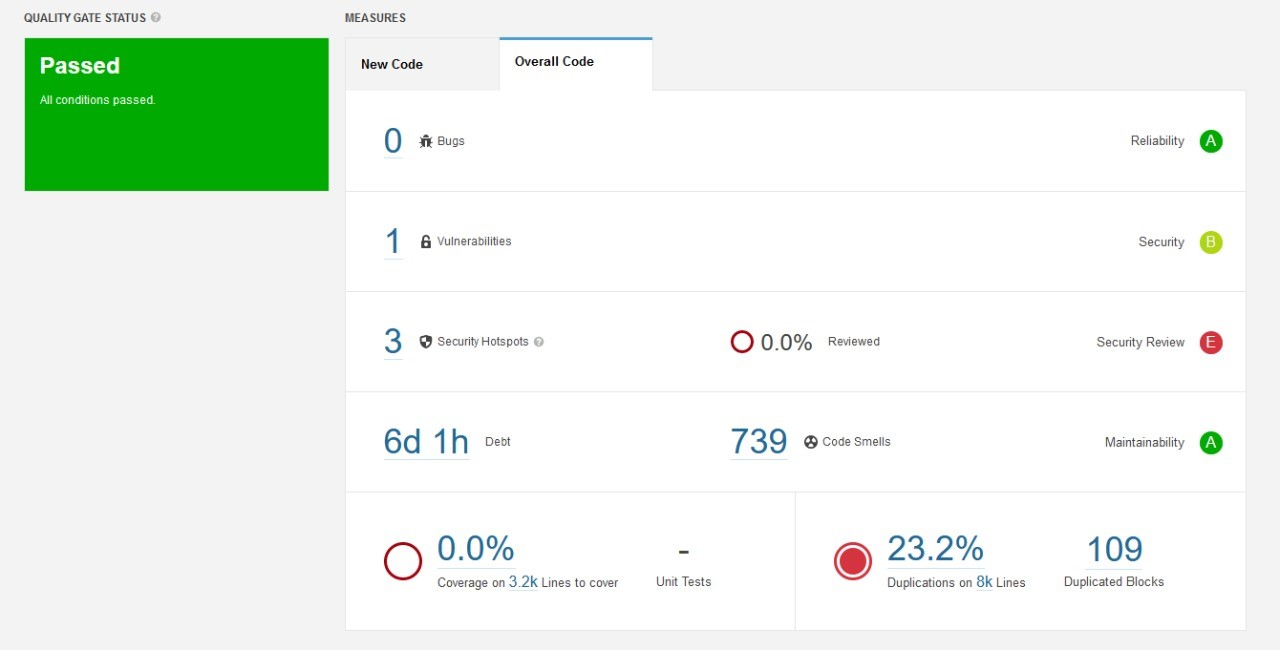
\includegraphics[width=15cm]{./img/image2.jpg} 
\end{center}
\begin{center}
	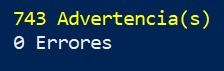
\includegraphics[width=10cm]{./img/image3.jpg} 
\end{center}

\textbf{VERSION MEJORADA}
\\
Resultados de las pruebas hechas en SONARQUBE despues de realizar las mejoras indicadas por el docente
\\
\begin{center}
	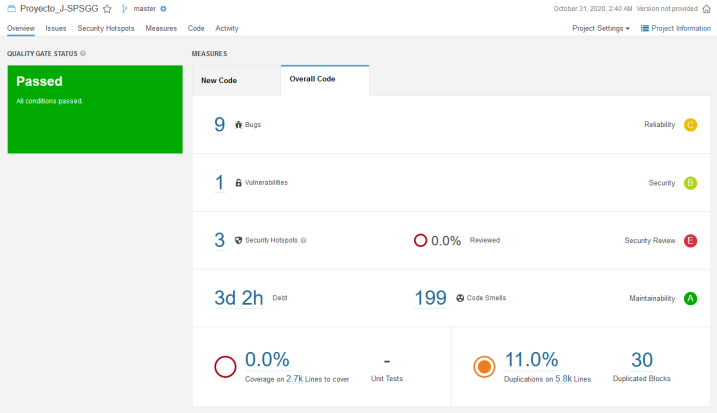
\includegraphics[width=15cm]{./img/image4.png} 
\end{center}
Muestra errores en Hotspot aun sin corregir(Nivel de error alto)
\\
\begin{center}
	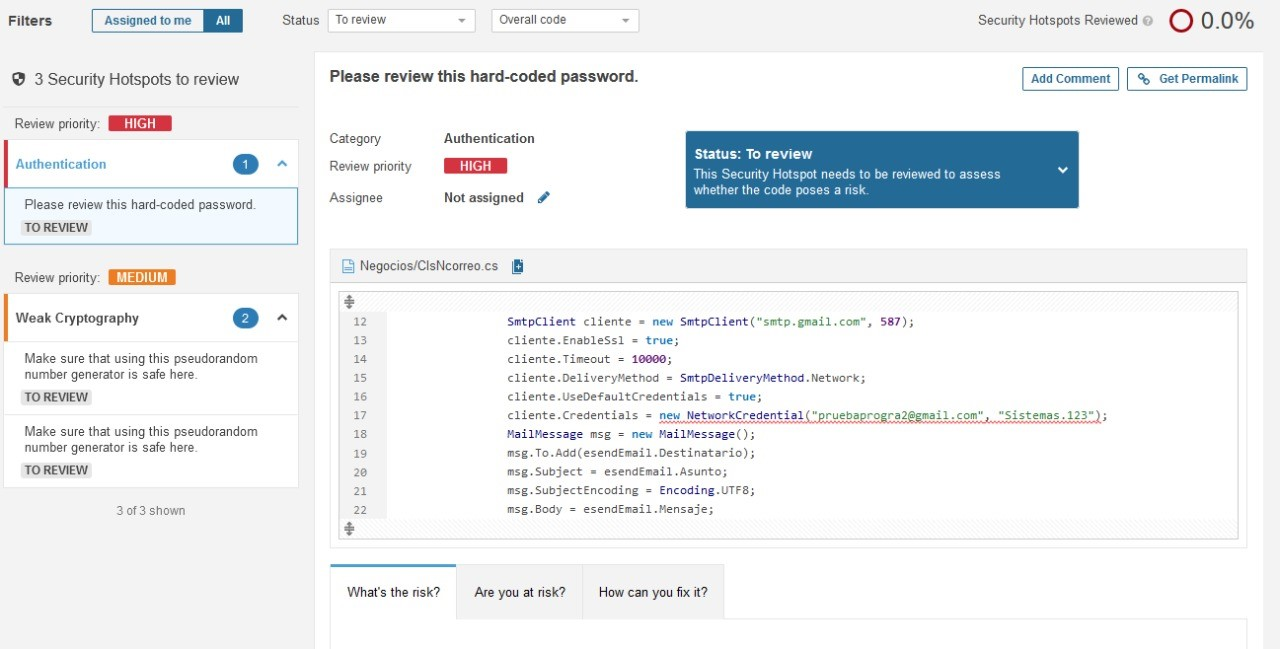
\includegraphics[width=15cm]{./img/image5.jpg} 
\end{center}
Muestra errores en Hotspot aun sin corregir(Nivel de error medio)
\\
\begin{center}
	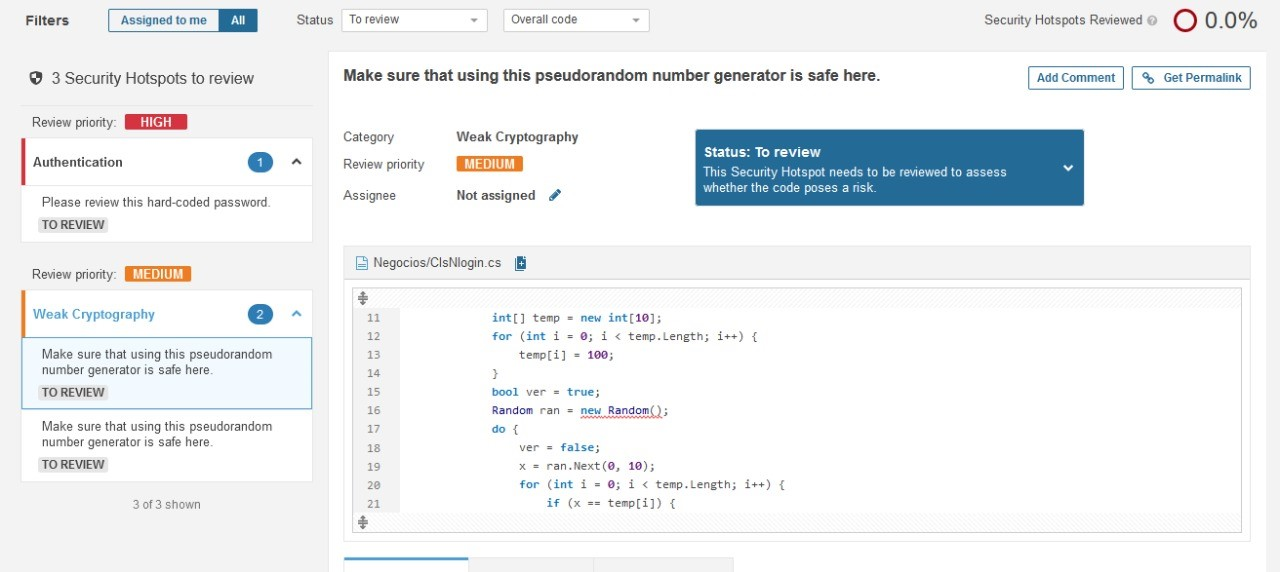
\includegraphics[width=15cm]{./img/image6.jpg} 
\end{center}
Muestra vulnerabilidades en el codigo
\\
\begin{center}
	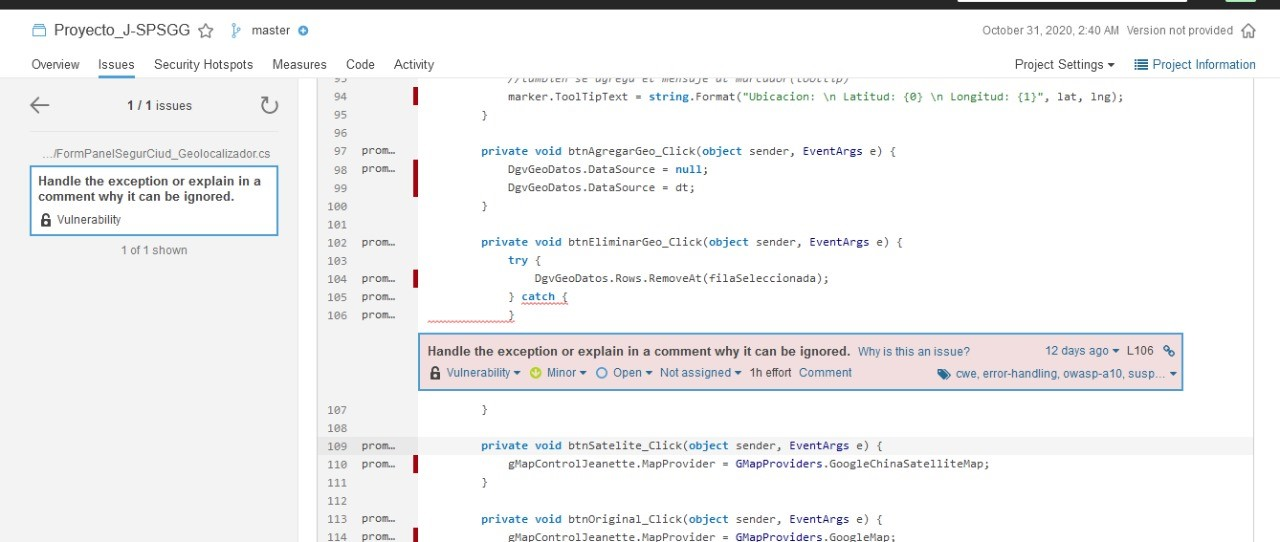
\includegraphics[width=15cm]{./img/image7.jpg} 
\end{center}
\begin{center}
	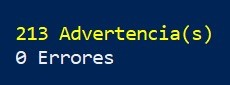
\includegraphics[width=10cm]{./img/image8.jpg} 
\end{center}

\subsection{Metodología, técnicas usadas}
\textbf{Singleton}
\\
Singleton es un patrón de diseño del tipo creacional cuyo propósito es garantizar la existencia de una sola instancia de una clase. Además el acceso a esa única instancia tiene que ser global.
En C\# la instrucción que contiene la palabra “new” sólo se puede ejecutar una vez, así nos aseguramos que sólo existe una instancia.
\\
\begin{center}
	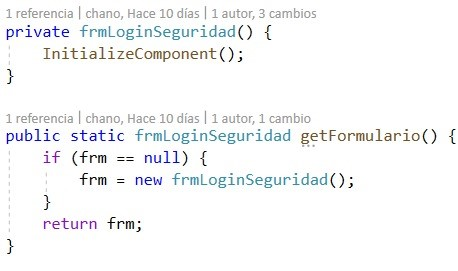
\includegraphics[width=10cm]{./img/image9.jpg} 
\end{center}

\textbf{Abstracciones}
\\
La abstracción es resumir o disminuir un elemento a lo que lo define sin incluir otros elementos, en este caso los objetos de la Programación Orientada a Objetos (POO).
Camel case
Es un estilo de escritura que se aplica a frases o palabras compuestas. El nombre se debe a que las mayúsculas a lo largo de una palabra en CamelCase se asemejan a las jorobas de un camello. El nombre CamelCase se podría traducir como Mayúsculas/Minúsculas Camello. El término case se traduce como "caja tipográfica", que a su vez implica si una letra es mayúscula o minúscula y tiene su origen en la disposición de los tipos móviles en casilleros o cajas.
\\
\begin{center}
	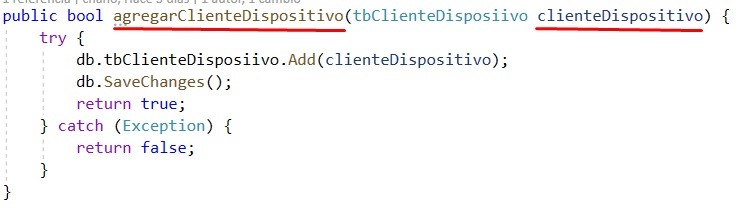
\includegraphics[width=10cm]{./img/image10.jpg} 
\end{center}

\textbf{Encapsulación}
\\
La encapsulación significa que un grupo de propiedades, métodos y otros miembros relacionados se tratan como una sola unidad u objeto.
\\
\begin{center}
	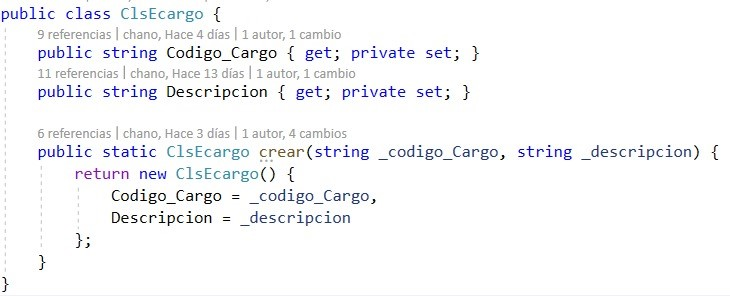
\includegraphics[width=10cm]{./img/image11.jpg} 
\end{center}

\textbf{ENTITI FRAMEWORK}
\\
Entity framework (en adelante, EF) es el marco ORM (mapeo relacional de objetos) que Microsoft pone a disposición como parte del desarrollo de .NET (versión 3.5 SP1 y posteriores). Su propósito es abstraer los vínculos con una base de datos relacional, de tal manera que el desarrollador pueda relacionarse con la entidad de la base de datos como un conjunto de objetos y luego con clases además de sus propiedades.
\\
\begin{center}
	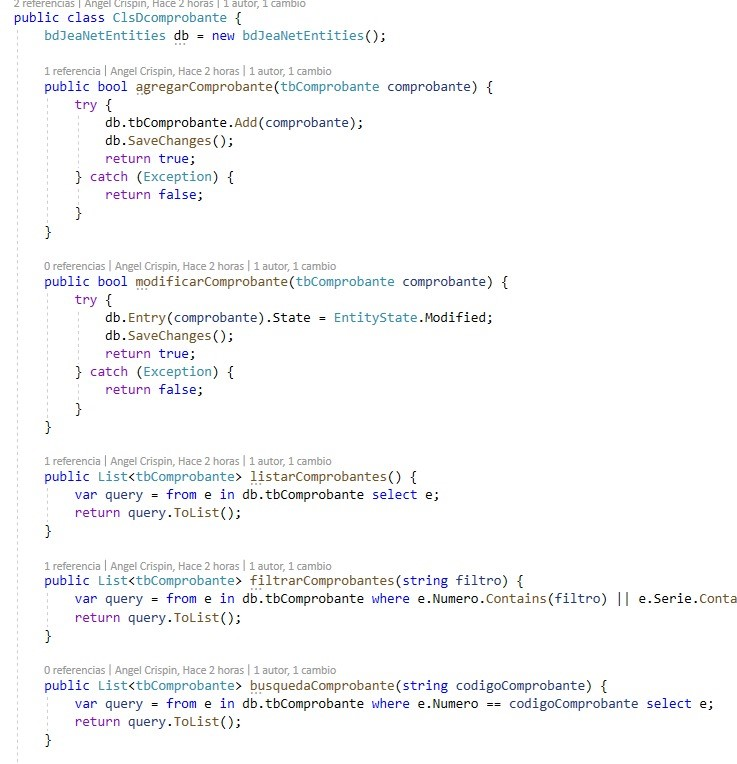
\includegraphics[width=10cm]{./img/image12.jpg} 
\end{center}

\textbf{INGENIERIA INVERSA}
\\
Las características para la ingeniería inversa todavía están en fase de desarrollo. " Una vista previa temprana de ingeniería inversa de un modelo de una base de datos ".
\\
\begin{center}
	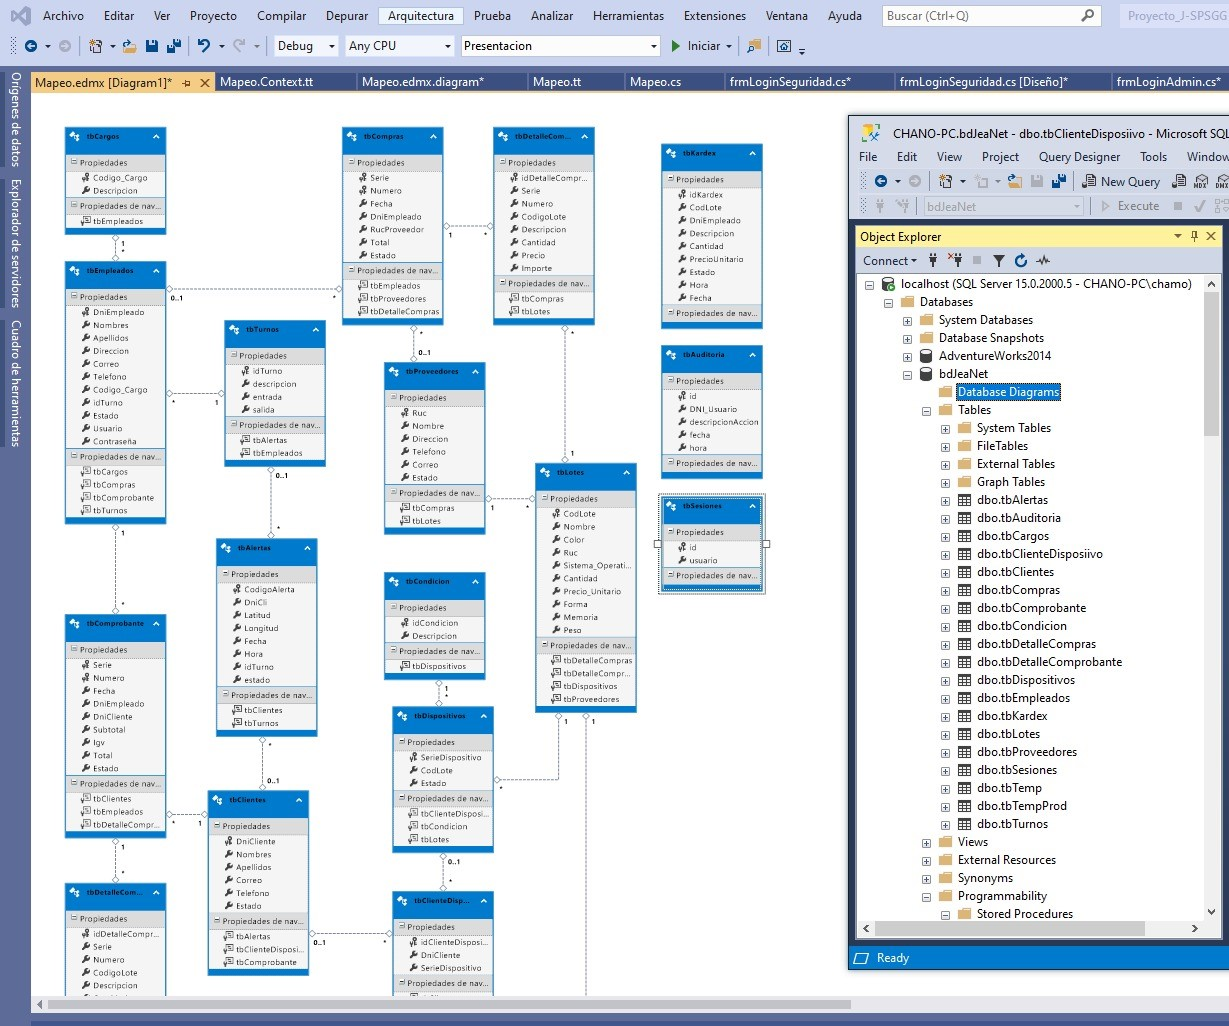
\includegraphics[width=10cm]{./img/image13.jpg} 
\end{center}

\textbf{PATRON FACTORY }
\\
El patrón de diseño Factory Method nos permite la creación de un subtipo determinado por medio de una clase de Factoría, la cual oculta los detalles de creación del objeto.
\\
\begin{center}
	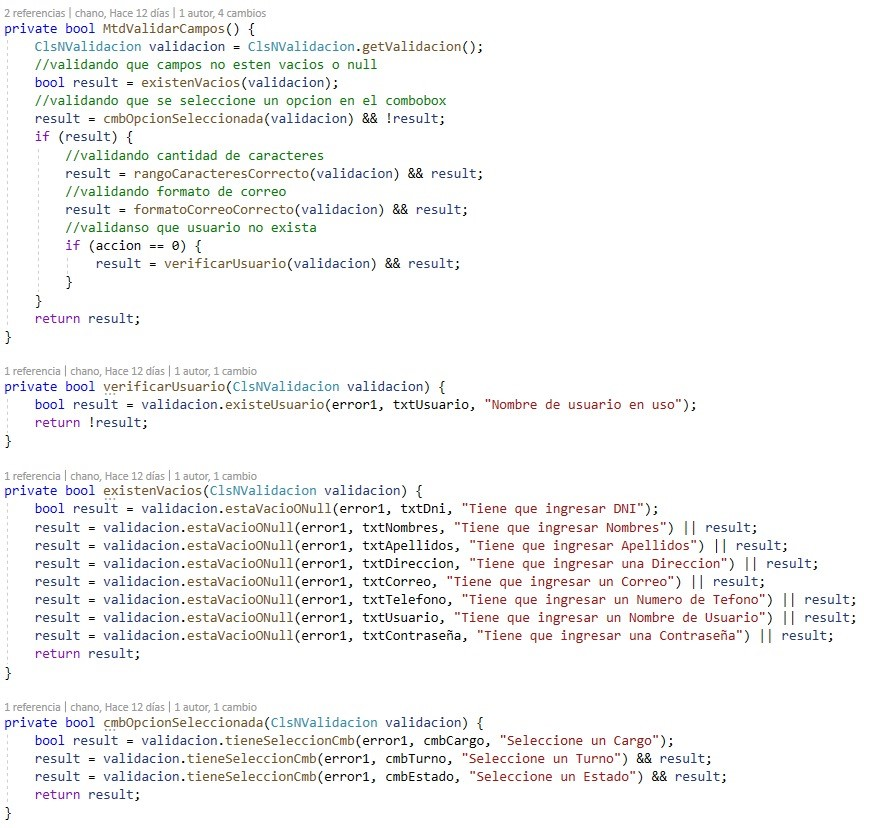
\includegraphics[width=10cm]{./img/image14.jpg} 
\end{center}
\begin{center}
	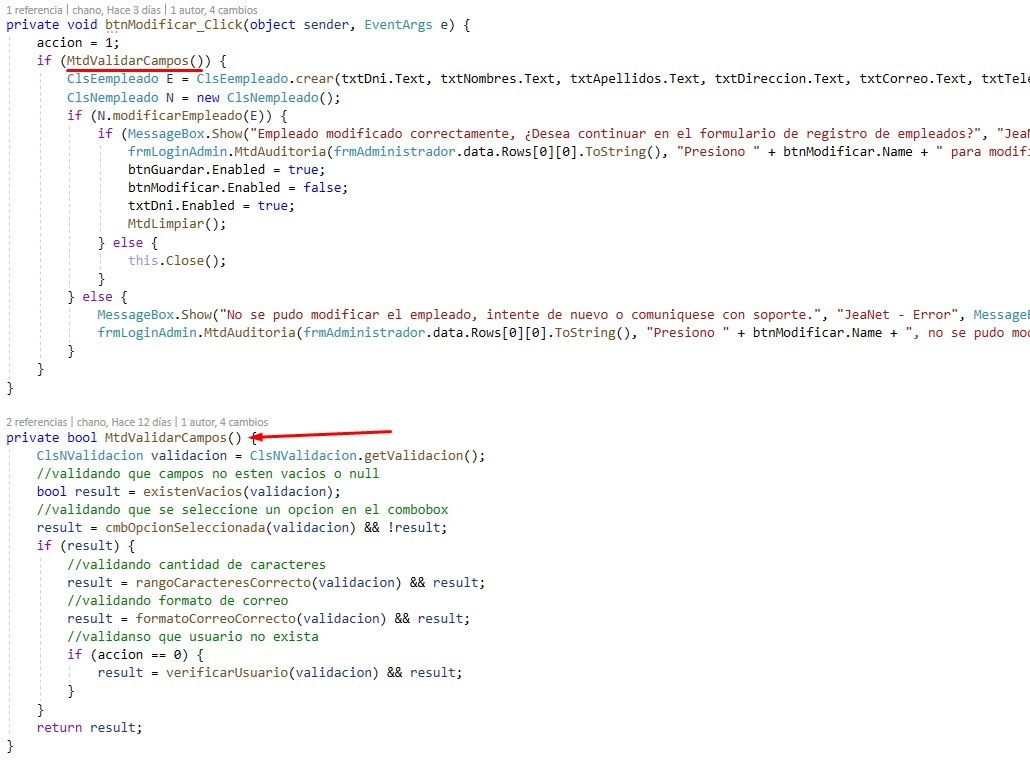
\includegraphics[width=10cm]{./img/image15.jpg} 
\end{center}

\subsection{Aplicación}
\subsubsection{Código de llamada al OR/M}
\begin{center}
	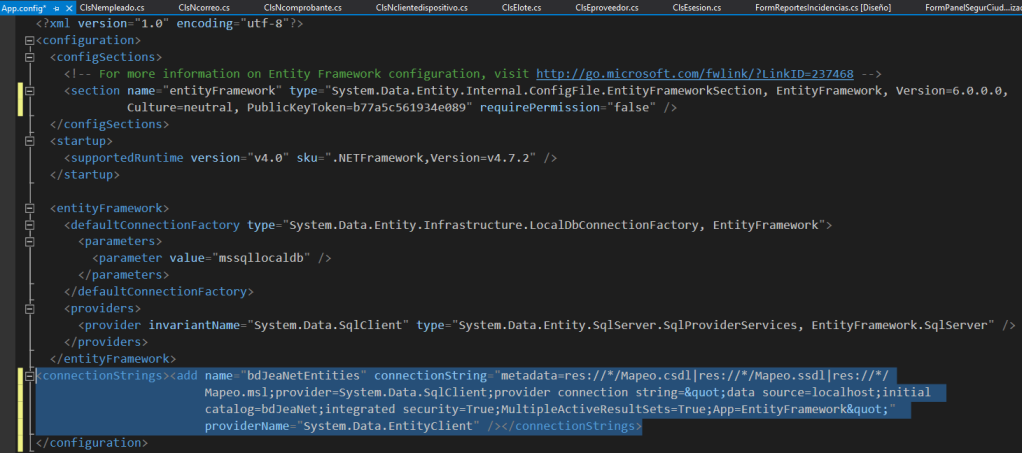
\includegraphics[width=15cm]{./img/image16.png} 
\end{center}
\subsubsection{Mapeo de objeto-relacional}
\begin{center}
	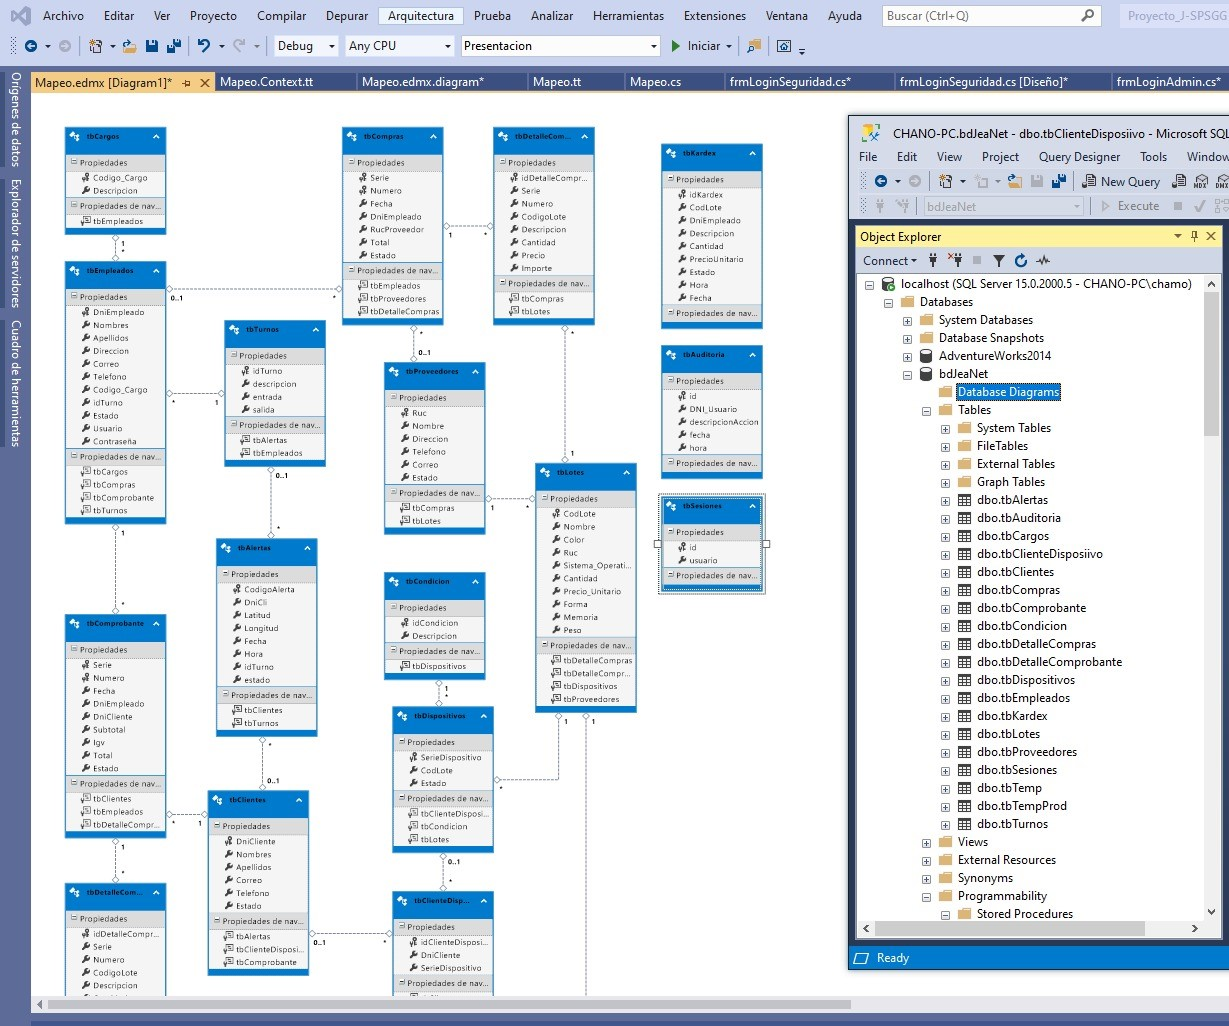
\includegraphics[width=15cm]{./img/image17.jpg} 
\end{center}


\subsubsection{Diccionario de datos}

%No relaciones
\begin{table}[t]
    \textbf{Nombre de la Tabla: } tbKardex\\
    \textbf{Descripción:} La tabla "tbKardex" contendrá información de compra y venta de productos, datos del empleado que realizó dicha acción, los datos del producto y fecha.\\
    \\
    \begin{tabular}{ | >{\centering\arraybackslash}m{2.5cm}  | >{\centering\arraybackslash}m{2cm}  | >{\centering\arraybackslash}m{2cm}  | >{\centering\arraybackslash}m{1.5cm}  | >{\centering\arraybackslash}m{1cm}  | m{7cm}  | }
        \hline
        \textbf{CAMPO} & \textbf{TIPO DE DATO} & \textbf{TAMAÑO} & \textbf{IS NULL} & \textbf{IS IDENTITY} & \textbf{DESCRIPCION}\\ \hline
        idKardex & bigint & 8 & NO & SI & Clave Única de Registro de Kardex \\ \hline
        CodLote & varchar & 4 & SI & NO & Código del lote del producto que está entrando o saliendo\\ \hline
        DniEmpleado & varchar & 8 & SI & NO & Dni del empleado que está realizando la entrada o salida de producto \\ \hline
        Descripcion & varchar & 255 & SI & NO & Descripción que guarda si se está registrando entrada o salida de productos \\ \hline
        Cantidad & int & 4 & SI & NO & Cantidad de productos que están entrando o saliendo \\ \hline
        PrecioUnitario & decimal & 9 & SI & NO & Precio unitario del producto que está entrando o saliendo \\ \hline
        Estado & varchar & 1 & SI & NO & Estado del Kardex, para saber si el Kardex es válido o esta anulado \\ \hline
        Hora & varchar & 10 & SI & NO & Hora en la que entran o salen productos \\ \hline
        Fecha & date & 3 & SI & NO & Fecha en la que entran o salen productos \\ \hline
    \end{tabular}
    \caption{Tabla Kardex}
\end{table}

\begin{table}[t]
    \textbf{Nombre de la Tabla: } tbAuditoria\\
    \textbf{Descripción:} La tabla "tbAuditoria" tendrá información de cada acción realizada dentro del sistema, el usuario de dicha acción, la fecha y la hora.\\
    \\
    \begin{tabular}{ | >{\centering\arraybackslash}m{2.5cm}  | >{\centering\arraybackslash}m{2cm}  | >{\centering\arraybackslash}m{2cm}  | >{\centering\arraybackslash}m{1.5cm}  | >{\centering\arraybackslash}m{1cm}  | m{7cm}  | }
        \hline
        \textbf{CAMPO} & \textbf{TIPO DE DATO} & \textbf{TAMAÑO} & \textbf{IS NULL} & \textbf{IS IDENTITY} & \textbf{DESCRIPCION}\\ \hline
        id & bigint & 8 & NO & YES & Clave Única de Registro de Auditoría \\ \hline
        DNI\_Usuario & varchar & 8 & YES & NO & Dni o Nombre de Usuario el cual realiza Acciones en el Sistema \\ \hline
        descripcion- Accion & varchar & 255 & YES & NO & Descripción de interacción de usuario con el sistema \\ \hline
        fecha & date & 3 & YES & NO & Fecha en la que se realiza la interacción del usuario con el sistema \\ \hline
        hora & varchar & 10 & YES & NO & Hora en la que se realiza la interacción del usuario con el sistema \\ \hline
    \end{tabular}
    \caption{Tabla Auditoria}
\end{table}

\begin{table}[t]
    \textbf{Nombre de la Tabla: } tbSesiones\\
    \textbf{Descripción:} La tabla "tbSesiones" tendrá información temporal sobre las cuentas activas en ese momento, para evitar dos cuentas activas al mismo tiempo.\\
    \\
    \begin{tabular}{ | >{\centering\arraybackslash}m{2.5cm}  | >{\centering\arraybackslash}m{2cm}  | >{\centering\arraybackslash}m{2cm}  | >{\centering\arraybackslash}m{1.5cm}  | >{\centering\arraybackslash}m{1cm}  | m{7cm}  | }
        \hline
        \textbf{CAMPO} & \textbf{TIPO DE DATO} & \textbf{TAMAÑO} & \textbf{IS NULL} & \textbf{IS IDENTITY} & \textbf{DESCRIPCION}\\ \hline
        Usuario & varchar & 20 & NO & NO & Nombre de usuario del empleado \\ \hline
        Contraseña & varchar & 6 & NO & NO & Contraseña de inicio de sesión del Empleado \\ \hline
    \end{tabular}
    \caption{Tabla Sesiones}
\end{table}

\begin{table}[t]
    \textbf{Nombre de la Tabla: } tbCargos\\
    \textbf{Descripción:} La tabla "tbCargos" tendrá información sobre los distintos tipos de cargos de la empresa.\\
    \\
    \begin{tabular}{ | >{\centering\arraybackslash}m{2.5cm}  | >{\centering\arraybackslash}m{2cm}  | >{\centering\arraybackslash}m{2cm}  | >{\centering\arraybackslash}m{1.5cm}  | >{\centering\arraybackslash}m{1cm}  | m{7cm}  | }
        \hline
        \textbf{CAMPO} & \textbf{TIPO DE DATO} & \textbf{TAMAÑO} & \textbf{IS NULL} & \textbf{IS IDENTITY} & \textbf{DESCRIPCION}\\ \hline
        Codigo\_Cargo & varchar & 3 & NO & NO & Clave Única de Registro de Cargo \\ \hline
        Descripcion & varchar & 50 & NO & NO & Descripción de cargo en el cual se desenvolverá el empleado \\ \hline
    \end{tabular}
    \caption{Tabla Auditoria}
\end{table}

\begin{table}[t]
    \textbf{Nombre de la Tabla: } tbClientes\\
    \textbf{Descripción:} La tabla "tbClientes" contendrá la información de todos los clientes de la empresa.\\
    \\
    \begin{tabular}{ | >{\centering\arraybackslash}m{2.5cm}  | >{\centering\arraybackslash}m{2cm}  | >{\centering\arraybackslash}m{2cm}  | >{\centering\arraybackslash}m{1.5cm}  | >{\centering\arraybackslash}m{1cm}  | m{7cm}  | }
        \hline
        \textbf{CAMPO} & \textbf{TIPO DE DATO} & \textbf{TAMAÑO} & \textbf{IS NULL} & \textbf{IS IDENTITY} & \textbf{DESCRIPCION}\\ \hline
        DniCliente & varchar & 8 & NO & NO & Clave Única de Registro de Cliente \\ \hline
        Nombres & varchar & 50 & NO & NO & Nombre del Cliente \\ \hline
        Apellidos & varchar & 50 & NO & NO & Apellido del Cliente \\ \hline
        Correo & varchar & 50 & NO & NO & Correo Electrónico del Cliente \\ \hline
        Telefono & varchar & 9 & NO & NO & Teléfono del Cliente \\ \hline
        Estado & varchar & 1 & NO & NO & Estado de Cliente, si es activo o inactivo \\ \hline
    \end{tabular}
    \caption{Tabla Clientes}
\end{table}

\begin{table}[t]
    \textbf{Nombre de la Tabla: } tbProveedores\\
    \textbf{Descripción:} La tabla "tbProveedores" tendrá toda la información de los proveedores de la empresa.\\
    \\
    \begin{tabular}{ | >{\centering\arraybackslash}m{2.5cm}  | >{\centering\arraybackslash}m{2cm}  | >{\centering\arraybackslash}m{2cm}  | >{\centering\arraybackslash}m{1.5cm}  | >{\centering\arraybackslash}m{1cm}  | m{7cm}  | }
        \hline
        \textbf{CAMPO} & \textbf{TIPO DE DATO} & \textbf{TAMAÑO} & \textbf{IS NULL} & \textbf{IS IDENTITY} & \textbf{DESCRIPCION}\\ \hline
        Ruc & varchar & 11 & NO & NO & Clave Única de Registro de Proveedores \\ \hline
        Nombre & varchar & 50 & NO & NO & Razón Social del Proveedor \\ \hline
        Direccion & varchar & 200 & NO & NO & Dirección del Proveedor \\ \hline
        Telefono & varchar & 9 & NO & NO & Teléfono del Proveedor \\ \hline
        Correo & varchar & 100 & NO & NO & Correo del Proveedor \\ \hline
        Estado & varchar & 1 & NO & NO & Estado del Proveedor, si está activo o inactivo \\ \hline
        id & bigint & 8 & NO & SI & Clave Única de Registro de Sesión \\ \hline
        usuario & varchar & 20 & SI & NO & Nombre de usuario que ha iniciado sesión \\ \hline
    \end{tabular}
    \caption{Tabla Proveedores}
\end{table}

\begin{table}[t]
    \textbf{Nombre de la Tabla: } tbTurnos\\
    \textbf{Descripción:} La tabla "tbTurnos" tendrá los tipos de turnos que tendrán los empleados de la empresa.\\
    \\
    \begin{tabular}{ | >{\centering\arraybackslash}m{2.5cm}  | >{\centering\arraybackslash}m{2cm}  | >{\centering\arraybackslash}m{2cm}  | >{\centering\arraybackslash}m{1.5cm}  | >{\centering\arraybackslash}m{1cm}  | m{7cm}  | }
        \hline
        \textbf{CAMPO} & \textbf{TIPO DE DATO} & \textbf{TAMAÑO} & \textbf{IS NULL} & \textbf{IS IDENTITY} & \textbf{DESCRIPCION}\\ \hline
        idTurno & int & 4 & NO & NO & Clave Única de identificación de Turno \\ \hline
        descripcion & varchar & 10 & NO & NO & Nombre del turno \\ \hline
        entrada & time & 5 & NO & NO & Hora de entrada del turno \\ \hline
        salida & time & 5 & NO & NO & Hora de salida del turno \\ \hline
    \end{tabular}
    \caption{Tabla Proveedores}
\end{table}

\begin{table}[t]
    \textbf{Nombre de la Tabla: } tbCondicion\\
    \textbf{Descripción:} La tabla "tbCondición" tendrá los tipos de condición que pueda tener un producto.\\
    \\
    \begin{tabular}{ | >{\centering\arraybackslash}m{2.5cm}  | >{\centering\arraybackslash}m{2cm}  | >{\centering\arraybackslash}m{2cm}  | >{\centering\arraybackslash}m{1.5cm}  | >{\centering\arraybackslash}m{1cm}  | m{7cm}  | }
        \hline
        \textbf{CAMPO} & \textbf{TIPO DE DATO} & \textbf{TAMAÑO} & \textbf{IS NULL} & \textbf{IS IDENTITY} & \textbf{DESCRIPCION}\\ \hline
        idCondicion & varchar & 1 & NO & NO & Clave Única de Registro de Condición \\ \hline
        Descripcion & varchar & 10 & NO & NO & Estado del Dispositivo: vendido, disponible, devuelto, malogrado, etc \\ \hline
    \end{tabular}
    \caption{Tabla Condicion}
\end{table}


%Si relaciones
\begin{table}[t]    
    \textbf{Nombre de la Tabla: } tbAlertas\\
    \textbf{Descripción:} La tabla "tbAlertas" tendrá todas las alertas que estarán realizando los usuarios.\\
    \\
    \begin{tabular}{ | >{\centering\arraybackslash}m{2.5cm}  | >{\centering\arraybackslash}m{2cm}  | >{\centering\arraybackslash}m{2cm}  | >{\centering\arraybackslash}m{1.5cm}  | >{\centering\arraybackslash}m{1cm}  | m{7cm}  | }
        \hline
        \textbf{CAMPO} & \textbf{TIPO DE DATO} & \textbf{TAMAÑO} & \textbf{IS NULL} & \textbf{IS IDENTITY} & \textbf{DESCRIPCION}\\ \hline
        CodigoAlerta & bigint & 8 & NO & YES & Clave Única de Registro de Alerta \\ \hline
        DniCli & varchar & 8 & YES & NO & Clave Referencial del Cliente que envía la Alerta \\ \hline
        Latitud & varchar & 50 & YES & NO & Latitud desde donde es enviada la Alerta \\ \hline
        Longitud & varchar & 50 & YES & NO & Longitud desde donde es enviada la Alerta \\ \hline
        Fecha & date & 3 & YES & NO & Fecha en la cual se envía la Alerta \\ \hline
        Hora & varchar & 10 & YES & NO & Hora en la cual se envía la Alerta \\ \hline
        idTurno & int & 4 & YES & NO & Clave Referencial del Turno en la cual es enviada la Alerta \\ \hline
        estado & varchar & 1 & YES & NO & Estado de la Alerta, si es aceptada o rechazada \\ \hline
    \end{tabular}
    \caption{Tabla Alertas}
    \textbf{Referencias: } \\
    • DniCli con tbClientes\\
    • idTurno con tbTurnos\\
\end{table}

\begin{table}[t]    
    \textbf{Nombre de la Tabla: } tbClienteDisposiivo\\
    \textbf{Descripción:} La tabla "tbClienteDisposiivo" tiene información de un producto con su respectivo cliente que realizó la compra.\\
    \\
    \begin{tabular}{ | >{\centering\arraybackslash}m{2.5cm}  | >{\centering\arraybackslash}m{2cm}  | >{\centering\arraybackslash}m{2cm}  | >{\centering\arraybackslash}m{1.5cm}  | >{\centering\arraybackslash}m{1cm}  | m{7cm}  | }
        \hline
        \textbf{CAMPO} & \textbf{TIPO DE DATO} & \textbf{TAMAÑO} & \textbf{IS NULL} & \textbf{IS IDENTITY} & \textbf{DESCRIPCION}\\ \hline
        idClienteDispositivo & bigint & 8 & NO & YES & Clave Única de Registro del Cliente con Dispositivo \\ \hline
        DniCliente & varchar & 8 & YES & NO & Clave Referencial del Cliente que compra el dispositivo \\ \hline
        SerieDispositivo & varchar & 9 & YES & NO & Clave Referencial del Dispositivo que se le vendió al Cliente \\ \hline
    \end{tabular}
    \caption{Tabla ClienteDispositivo}
    \textbf{Referencias: } \\
    • DniCliente con tbClientes\\
    • SerieDispositivo con tbDispositivos\\
\end{table}

\begin{table}[t]    
    \textbf{Nombre de la Tabla: } tbCompras\\
    \textbf{Descripción:} La tabla "tbCompras" tiene toda la información del as compras realizadas de la empresa.\\
    \\
    \begin{tabular}{ | >{\centering\arraybackslash}m{2.5cm}  | >{\centering\arraybackslash}m{2cm}  | >{\centering\arraybackslash}m{2cm}  | >{\centering\arraybackslash}m{1.5cm}  | >{\centering\arraybackslash}m{1cm}  | m{7cm}  | }
        \hline
        \textbf{CAMPO} & \textbf{TIPO DE DATO} & \textbf{TAMAÑO} & \textbf{IS NULL} & \textbf{IS IDENTITY} & \textbf{DESCRIPCION}\\ \hline
        Serie & varchar & 3 & NO & NO & Clave Única de Registro de Serie de la Compra \\ \hline
        Numero & varchar & 6 & NO & NO & Clave Única de Registro de Numero de la Compra \\ \hline
        Fecha & date & 3 & YES & NO & Fecha en la cual es realizada la Compra \\ \hline
        DniEmpleado & varchar & 8 & YES & NO & Clave Referencial del Empleado que realiza la Compra \\ \hline
        RucProveedor & varchar & 11 & YES & NO & Clave Referencial del Proveedor al que se le Compra \\ \hline
        Total & decimal & 9 & YES & NO & Monto Total de la Compra \\ \hline
        Estado & varchar & 1 & YES & NO & Estado para saber si la Compra es válida o esta anulada \\ \hline
    \end{tabular}
    \caption{Tabla Compras}
    \textbf{Referencias: } \\
    • DniEmpleado con tbEmpleados\\
    • RucProveedor con tbProveedores\\
\end{table}

\begin{table}[t]    
    \textbf{Nombre de la Tabla: } tbComprobante\\
    \textbf{Descripción:} La tabla "tbComprobante" tiene toda la información de las ventas de la empresa.\\
    \\
    \begin{tabular}{ | >{\centering\arraybackslash}m{2.5cm}  | >{\centering\arraybackslash}m{2cm}  | >{\centering\arraybackslash}m{2cm}  | >{\centering\arraybackslash}m{1.5cm}  | >{\centering\arraybackslash}m{1cm}  | m{7cm}  | }
        \hline
        \textbf{CAMPO} & \textbf{TIPO DE DATO} & \textbf{TAMAÑO} & \textbf{IS NULL} & \textbf{IS IDENTITY} & \textbf{DESCRIPCION}\\ \hline
        Serie & varchar & 3 & NO & NO & Clave Única de Registro de Serie de Comprobante \\ \hline
        Numero & varchar & 6 & NO & NO & Clave Única de Registro de Numero de Comprobante \\ \hline
        Fecha & date & 3 & NO & NO & Fecha en la cual es emitido el Comprobante \\ \hline
        DniEmpleado & varchar & 8 & NO & NO & Clave Referencial del Empleado que realiza el Comprobante \\ \hline
        DniCliente & varchar & 8 & NO & NO & Clave Referencial del Cliente el cual recibe el Comprobante \\ \hline
        Subtotal & decimal & 9 & NO & NO & Sub-Total de lo comprado en el Comprobante \\ \hline
        Igv & decimal & 9 & NO & NO & Impuesto General a la Venta del monto Sub-Total \\ \hline
        Total & decimal & 9 & NO & NO & Total del Comprobante, la suma del IGV más el Sub-Total \\ \hline
        Estado & varchar & 1 & YES & NO & Estado para saber si el Comprobante es válido o está anulado \\ \hline
    \end{tabular}
    \caption{Tabla Comprobante}
    \textbf{Referencias: } \\
    • DniEmpleado con tbEmpleados\\
    • DniCliente con tbClientes\\
\end{table}

\begin{table}[t]    
    \textbf{Nombre de la Tabla: } tbDetalleCompras\\
    \textbf{Descripción:} La tabla "tbDetalleCompras" tiene la información de los detalles de los productos realizados en una compra de la empresa.\\
    \\
    \begin{tabular}{ | >{\centering\arraybackslash}m{2.5cm}  | >{\centering\arraybackslash}m{2cm}  | >{\centering\arraybackslash}m{2cm}  | >{\centering\arraybackslash}m{1.5cm}  | >{\centering\arraybackslash}m{1cm}  | m{7cm}  | }
        \hline
        \textbf{CAMPO} & \textbf{TIPO DE DATO} & \textbf{TAMAÑO} & \textbf{IS NULL} & \textbf{IS IDENTITY} & \textbf{DESCRIPCION}\\ \hline
        idDetalleComprobante & bigint & 8 & NO & YES & Clave Única de Registro de Detalle de Comprobante \\ \hline
        Serie & varchar & 3 & NO & NO & Clave Referencial a la Serie del Comprobante \\ \hline
        Numero & varchar & 6 & NO & NO & Clave Referencial al Número del Comprobante \\ \hline
        CodigoLote & varchar & 4 & NO & NO & Clave Referencial del lote al que corresponde el producto que se está comprando \\ \hline
        Descripcion & varchar & 100 & NO & NO & Descripción del producto que se compra \\ \hline
        Cantidad & int & 4 & NO & NO & Cantidad del producto que se compra \\ \hline
        Precio & decimal & 9 & NO & NO & Precio unitario del producto que se compra \\ \hline
        Importe & decimal & 9 & NO & NO & Total a pagar por el producto, la cantidad por el precio \\ \hline
    \end{tabular}
    \caption{Tabla DetalleCompras}
    \textbf{Referencias: } \\
    • Serie con tbCompras\\
    • Numero con tbCompras\\
    • CodigoLote con tbLotes\\
\end{table}

\begin{table}[t]    
    \textbf{Nombre de la Tabla: } tbDetalleComprobante\\
    \textbf{Descripción:} La tabla "tbDetalleCompras" tiene la información de los detalles de los productos realizados en una venta de la empresa.\\
    \\
    \begin{tabular}{ | >{\centering\arraybackslash}m{2.5cm}  | >{\centering\arraybackslash}m{2cm}  | >{\centering\arraybackslash}m{2cm}  | >{\centering\arraybackslash}m{1.5cm}  | >{\centering\arraybackslash}m{1cm}  | m{7cm}  | }
        \hline
        \textbf{CAMPO} & \textbf{TIPO DE DATO} & \textbf{TAMAÑO} & \textbf{IS NULL} & \textbf{IS IDENTITY} & \textbf{DESCRIPCION}\\ \hline
        idDetalleComprobante & bigint & 8 & NO & YES & Clave Única de Registro de DetalleComprobante \\ \hline
        Serie & varchar & 3 & NO & NO & Clave Referencial a la Serie del Comprobante \\ \hline
        Numero & varchar & 6 & NO & NO & Clave Referencial al Número del Comprobante \\ \hline
        CodigoLote & varchar & 4 & NO & NO & Clave Referencial del lote al que corresponde el producto que se está vendiendo \\ \hline
        Descripcion & varchar & 100 & NO & NO & Descripción del producto que se vende \\ \hline
        Cantidad & int & 4 & NO & NO & Cantidad del producto que se vende \\ \hline
        Precio & decimal & 9 & NO & NO & Precio unitario del producto que se vende \\ \hline
        Importe & decimal & 9 & NO & NO & Total a pagar por el producto, la cantidad por el precio \\ \hline
    \end{tabular}
    \caption{Tabla DetalleComprobante}
    \textbf{Referencias: } \\
    • Serie con tbComprobante\\
    • Numero con tbComprobante\\
    • CodigoLote con tbLotes\\
\end{table}

\begin{table}[t]    
    \textbf{Nombre de la Tabla: } tbDispositivos\\
    \textbf{Descripción:} La tabla "tbDispositivos" contiene información general de los productos de la empresa.\\
    \\
    \begin{tabular}{ | >{\centering\arraybackslash}m{2.5cm}  | >{\centering\arraybackslash}m{2cm}  | >{\centering\arraybackslash}m{2cm}  | >{\centering\arraybackslash}m{1.5cm}  | >{\centering\arraybackslash}m{1cm}  | m{7cm}  | }
        \hline
        \textbf{CAMPO} & \textbf{TIPO DE DATO} & \textbf{TAMAÑO} & \textbf{IS NULL} & \textbf{IS IDENTITY} & \textbf{DESCRIPCION}\\ \hline
        SerieDispositivo & varchar & 9 & NO & NO & Referencia Única de Registro de Dispositivo \\ \hline
        CodLote & varchar & 4 & NO & NO & Clave Referencial del Lote al que pertenece el Dispositivo \\ \hline
        Estado & varchar & 1 & NO & NO & Clave Referencial de la Condición del Dispositivo \\ \hline
    \end{tabular}
    \caption{Tabla Alertas}
    \textbf{Referencias: } \\
    • CodLote con tbLotes\\
    • Estado con tbCondicion\\
\end{table}

\begin{table}[t]    
    \textbf{Nombre de la Tabla: } tbEmpleados\\
    \textbf{Descripción:} La tabla "tbEmpleados" tiene la información de los empleados de la empresa.\\
    \\
    \begin{tabular}{ | >{\centering\arraybackslash}m{2.5cm}  | >{\centering\arraybackslash}m{2cm}  | >{\centering\arraybackslash}m{2cm}  | >{\centering\arraybackslash}m{1.5cm}  | >{\centering\arraybackslash}m{1cm}  | m{7cm}  | }
        \hline
        \textbf{CAMPO} & \textbf{TIPO DE DATO} & \textbf{TAMAÑO} & \textbf{IS NULL} & \textbf{IS IDENTITY} & \textbf{DESCRIPCION}\\ \hline
        DniEmpleado & varchar & 8 & NO & NO & Clave Única de Registro de Empleado \\ \hline
        Nombres & varchar & 50 & NO & NO & Nombres del Empleado \\ \hline
        Apellidos & varchar & 50 & NO & NO & Apellidos del Empleado \\ \hline
        Direccion & varchar & 100 & NO & NO & Dirección del Empleado \\ \hline
        Correo & varchar & 100 & NO & NO & Correo del Empleado \\ \hline
        Telefono & varchar & 9 & NO & NO & Teléfono del Empleado \\ \hline
        Codigo\_Cargo & varchar & 3 & NO & NO & Clave Referencial del Cargo que tiene el Empleado \\ \hline
        idTurno & int & 4 & NO & NO & Clave Referencial del Turno del Empleado \\ \hline
        Estado & varchar & 1 & NO & NO & Estado del Empleado, si está activo o inactivo \\ \hline
    \end{tabular}
    \caption{Tabla Empleados}
    \textbf{Referencias: } \\
    • Codigo\_Cargo con tbCargos\\
    • idTurno con tbTurnos\\
\end{table}

\begin{table}[t]    
    \textbf{Nombre de la Tabla: } tbLotes\\
    \textbf{Descripción:} La tabla "tbLotes" contiene la información detallada de los productos.\\
    \\
    \begin{tabular}{ | >{\centering\arraybackslash}m{2.5cm}  | >{\centering\arraybackslash}m{2cm}  | >{\centering\arraybackslash}m{2cm}  | >{\centering\arraybackslash}m{1.5cm}  | >{\centering\arraybackslash}m{1cm}  | m{7cm}  | }
        \hline
        \textbf{CAMPO} & \textbf{TIPO DE DATO} & \textbf{TAMAÑO} & \textbf{IS NULL} & \textbf{IS IDENTITY} & \textbf{DESCRIPCION}\\ \hline
        CodLote & varchar & 4 & NO & NO & Clave Única de Registro de Lote \\ \hline
        Nombre & varchar & 50 & NO & NO & Nombre del lote \\ \hline
        Color & varchar & 20 & NO & NO & Color de cada dispositivo del lote \\ \hline
        Ruc & varchar & 11 & NO & NO & Clave Referencial del proveedor que vende el lote \\ \hline
        Sistema\_Operativo & varchar & 20 & NO & NO & Sistema operativo de todos los dispositivos del lote \\ \hline
        Cantidad & int & 4 & NO & NO & Cantidad de dispositivos que trae el lote \\ \hline
        Precio\_Unitario & decimal & 9 & NO & NO & Precio unitario de cada dispositivo del lote \\ \hline
        Forma & varchar & 50 & NO & NO & Forma que tienen todos los dispositivos del lote \\ \hline
        Memoria & varchar & 10 & NO & NO & Memoria que tienen todos los dispositivos del lote \\ \hline
        Peso & decimal & 9 & NO & NO & Peso de cada dispositivo del lote \\ \hline
    \end{tabular}
    \caption{Tabla Lotes}
    \textbf{Referencias: } \\
    • Ruc con tbProveedores\\
\end{table}

\begin{table}[t]    
    \textbf{Nombre de la Tabla: } tbTemp\\
    \textbf{Descripción:} La tabla "tbTemp" es una tabla temporal, que se usa para obtener un reporte detallado sobre las ventas de los empleados.\\
    \\
    \begin{tabular}{ | >{\centering\arraybackslash}m{2.5cm}  | >{\centering\arraybackslash}m{2cm}  | >{\centering\arraybackslash}m{2cm}  | >{\centering\arraybackslash}m{1.5cm}  | >{\centering\arraybackslash}m{1cm}  | m{7cm}  | }
        \hline
        \textbf{CAMPO} & \textbf{TIPO DE DATO} & \textbf{TAMAÑO} & \textbf{IS NULL} & \textbf{IS IDENTITY} & \textbf{DESCRIPCION}\\ \hline
        dni & varchar & 8 & SI & NO & Clave Referencial del Empleado que realizo la venta \\ \hline
        dia & int & 4 & SI & NO & Dia en que se realizó la venta el empleado \\ \hline
        valor & decimal & 9 & SI & NO & Monto de la venta que realizo la venta el Empleado \\ \hline
    \end{tabular}
    \caption{Tabla Temporal Empleados}
    \textbf{Referencias: } \\
    • dni con tbEmpleados\\
\end{table}

\begin{table}[t]    
    \textbf{Nombre de la Tabla: } tbTempProd\\
    \textbf{Descripción:} La tabla "tbTempProd" es una tabla temporal, que se usa para obtener un reporte detallado sobre los productos vendidos.
    \\
    \begin{tabular}{ | >{\centering\arraybackslash}m{2.5cm}  | >{\centering\arraybackslash}m{2cm}  | >{\centering\arraybackslash}m{2cm}  | >{\centering\arraybackslash}m{1.5cm}  | >{\centering\arraybackslash}m{1cm}  | m{7cm}  | }
        \hline
        \textbf{CAMPO} & \textbf{TIPO DE DATO} & \textbf{TAMAÑO} & \textbf{IS NULL} & \textbf{IS IDENTITY} & \textbf{DESCRIPCION}\\ \hline
        CodigoLote & varchar & 4 & SI & NO & Clave Referencial del código del lote que se vende el producto \\ \hline
        dia & int & 4 & SI & NO & Dia en que se realizó la venta del Producto \\ \hline
        valor & bigint & 8 & SI & NO & Valor de la venta del Producto \\ \hline
    \end{tabular}
    \caption{Tabla Temporal Productos}
    \textbf{Referencias: } \\
    • CodigoLote con tbLotes\\
\end{table}
%%%%%%%%%%%%%%%%%%%%%%%%%%%%%%%%%%%%%%%%%%%%%%%%%%%%%%%%%
\end{document}